%% LaTeX Paper Template, Flip Tanedo (flip.tanedo@ucr.edu)
%% last updated: Dec 2016

\documentclass[12pt]{article}

%%%%%%%%%%%%%%%%%%%%%%%%%%
%%%  COMMON PACKAGES  %%%%
%%%%%%%%%%%%%%%%%%%%%%%%%%

\usepackage{amsmath}
\usepackage{amssymb}
\usepackage{amsfonts}
\usepackage{graphicx}
\usepackage[utf8]{inputenc}	% for inspirehep.net bibs
 

%%%%%%%%%%%%%%%%%%%%%%%%%%%%%%%%%
%%%  UNUSUAL PACKAGES        %%%%
%%%  Uncomment as necessary. %%%%
%%%%%%%%%%%%%%%%%%%%%%%%%%%%%%%%%

%% MATH AND PHYSICS SYMBOLS
%% ------------------------
\usepackage{slashed}       % \slashed{k}
\usepackage{mathrsfs}      % Weinberg-esque letters
\usepackage{pifont}        % check marks
\usepackage{bbm}           % \mathbbm{1} incomp. w/ XeLaTeX 
\usepackage{cancel}		   % for slashed words

%% CONTENT FORMAT AND DESIGN
%% -------------------------
\usepackage[dvipsnames]{xcolor} % color definitions
\usepackage{lipsum}         % block of text (formatting test)
%\usepackage{subcaption}    % subfigures; subfig depreciated
%\usepackage{cite}          % group cites (conflict: collref)
%\usepackage{xspace}			% spacing after macros


%% TABLES IN LaTeX
%% ---------------
\usepackage{booktabs}      % professional tables
\usepackage{nicefrac}      % fractions in tables,
\usepackage{multirow}      % multirow elements in a table
\usepackage{arydshln} 	    % dashed lines in arrays

%% Other Packages and Notes
%% ------------------------
\usepackage[font=small]{caption} % caption font is small
\usepackage{float}         % for strict placement e.g. [H]




%%%%%%%%%%%%%%%%%%%%%%%%%%%%%%
%%%  DOCUMENT PROPERTIES  %%%%
%%%%%%%%%%%%%%%%%%%%%%%%%%%%%%
\usepackage[margin=2cm]{geometry}   % margins
\graphicspath{{figures/}}			% figure folder
\numberwithin{equation}{section}    % set equation numbering


% Change list spacing (instead of package paralist)
% from: http://en.wikibooks.org/wiki/LaTeX/List_Structures#Line_spacing
\let\oldenumerate\enumerate
\renewcommand{\enumerate}{
  \oldenumerate
  \setlength{\itemsep}{1pt}
  \setlength{\parskip}{0pt}
  \setlength{\parsep}{0pt}
}

\let\olditemize\itemize
\renewcommand{\itemize}{
  \olditemize
  \setlength{\itemsep}{1pt}
  \setlength{\parskip}{0pt}
  \setlength{\parsep}{0pt}
}


%%%%%%%%%%%%%%%%%%%%%%%%%%%
%%%  (RE)NEW COMMANDS  %%%%
%%%%%%%%%%%%%%%%%%%%%%%%%%%

%% COMMON PHYSICS MACROS
%% ---------------------
\renewcommand{\tilde}{\widetilde}   % tilde over characters
\renewcommand{\vec}[1]{\mathbf{#1}} % vectors are boldface
\newcommand{\dbar}{d\mkern-6mu\mathchar'26}    % for d/2pi
\newcommand{\ket}[1]{\left|#1\right\rangle}    % <#1|
\newcommand{\bra}[1]{\left\langle#1\right|}    % |#1>


%% COMMANDS FOR TOP-MATTER
%% -----------------------
\newcommand{\email}[1]{\href{mailto:#1}{#1}}
\newenvironment{institutions}[1][2em]{\begin{list}{}{\setlength\leftmargin{#1}\setlength\rightmargin{#1}}\item[]}{\end{list}}


%%%%%%%%%%%%%%%%%%%
%%%  HYPERREF  %%%%
%%%%%%%%%%%%%%%%%%%

%% This package has to be at the end; can lead to conflicts

\usepackage[
	colorlinks=true,
	citecolor=green!50!black,
	linkcolor=NavyBlue!75!black,
	urlcolor=green!50!black,
	hypertexnames=false]{hyperref}




%%%%%%%%%%%%%%%%%%%%
%%%  BEGIN DOC  %%%%
%%%%%%%%%%%%%%%%%%%%



\begin{document}

\thispagestyle{empty}		% no page number on first page

\begin{center}

    {\huge \bf Clever Paper Title}

    \vskip .7cm

%% SINGLE AUTHOR FORMAT
%% --------------------
	\textbf{Flip Tanedo} \\
	\texttt{\footnotesize \email{flip.tanedo@ucr.edu}}

	\vspace{-1em}
    \begin{institutions}[2.25cm]
    \footnotesize
    {\it 
	    Department of Physics \& Astronomy, 
	    University of  California, Riverside, 
	    {CA} 92521	    
	    }    
    \end{institutions}


%% MULTIPLE AUTHOR FORMAT
%% --------------------
%    { \bf 
%    	Philip Tanedo$^{a}$
%    	and 
%    	Another Author$^{b}$ 
%    	} 
%    \\ 
%    \vspace{-.2em}
%    { \tt \footnotesize
%	    \email{flip.tanedo@ucr.edu},
%	    \email{another.author@university.edu}
%    }
%	
%    \vspace{-.2cm}
%
%    \begin{institutions}[2.25cm]
%    \footnotesize
%    $^{a}$ 
%    {\it 
%	    Department of Physics \& Astronomy, 
%	    University of  California, Riverside, 
%	    {CA} 92521	    
%	    }    
%	\\ 
%	\vspace*{0.05cm}   
%	$^{b}$ 
%	{\it 
%        Department of Physics, 
%        University, 
%        University Town, CA 90210
%        }
%    \end{institutions}

\end{center}




%%%%%%%%%%%%%%%%%%%%%
%%%  ABSTRACT    %%%%
%%%%%%%%%%%%%%%%%%%%%

\begin{abstract}
\noindent 
This is a simple template for my papers. It's not very different from the plain article style, but it has most of the macros I use pre-written.
\end{abstract}



\small
\setcounter{tocdepth}{2}
\tableofcontents
\normalsize
%\clearpage


%%%%%%%%%%%%%%%%%%%%%
%%%  THE MEAT    %%%%
%%%%%%%%%%%%%%%%%%%%%



\section{Introduction}

All of my students should read my lectures on `beyond the Standard Model physics'~\cite{Csaki:2016kln}.

 
\section{Itemize test}

\begin{itemize}% \itemsep1pt \parskip0pt \parsep0pt
\item Item 1
\item Item 2
\item Item 3
\end{itemize}

\begin{enumerate}% \itemsep1pt \parskip0pt \parsep0pt
\item Item 1
\item Item 2
\item Item 3
\end{enumerate}

\section{Table Example}

 
\begin{table}
	\renewcommand{\arraystretch}{1.3} % spacing between rows
	\centering
	\begin{tabular}{ @{} llll @{} } \toprule % @{} removes space
		Element & Core MF & Mantle MF & $C_\text{cap}^N (\text{s}^{-1})$ 
		\\ \hline
		Iron & 0.855 & 0.0626 & $9.43\times 10^{7}$ 
		\\
		Nickel & 0.052 & 0.00196 & $7.10\times 10^{6}$ 
		\\
		Silicon & 0.06 & 0.210 & $2.24\times 10^{6}$ 
		\\
		Magnesium & 0 & 0.228 & $1.05\times 10^{6}$ 
		\\ \bottomrule
	\end{tabular}
	\caption{
		Mass fractions of the Earth's core and mantle.
		\label{table:elements}
	}
\end{table}


 
\section{Lipsum}
 
 
 \lipsum[3-5]

\begin{figure}
	\begin{center}
		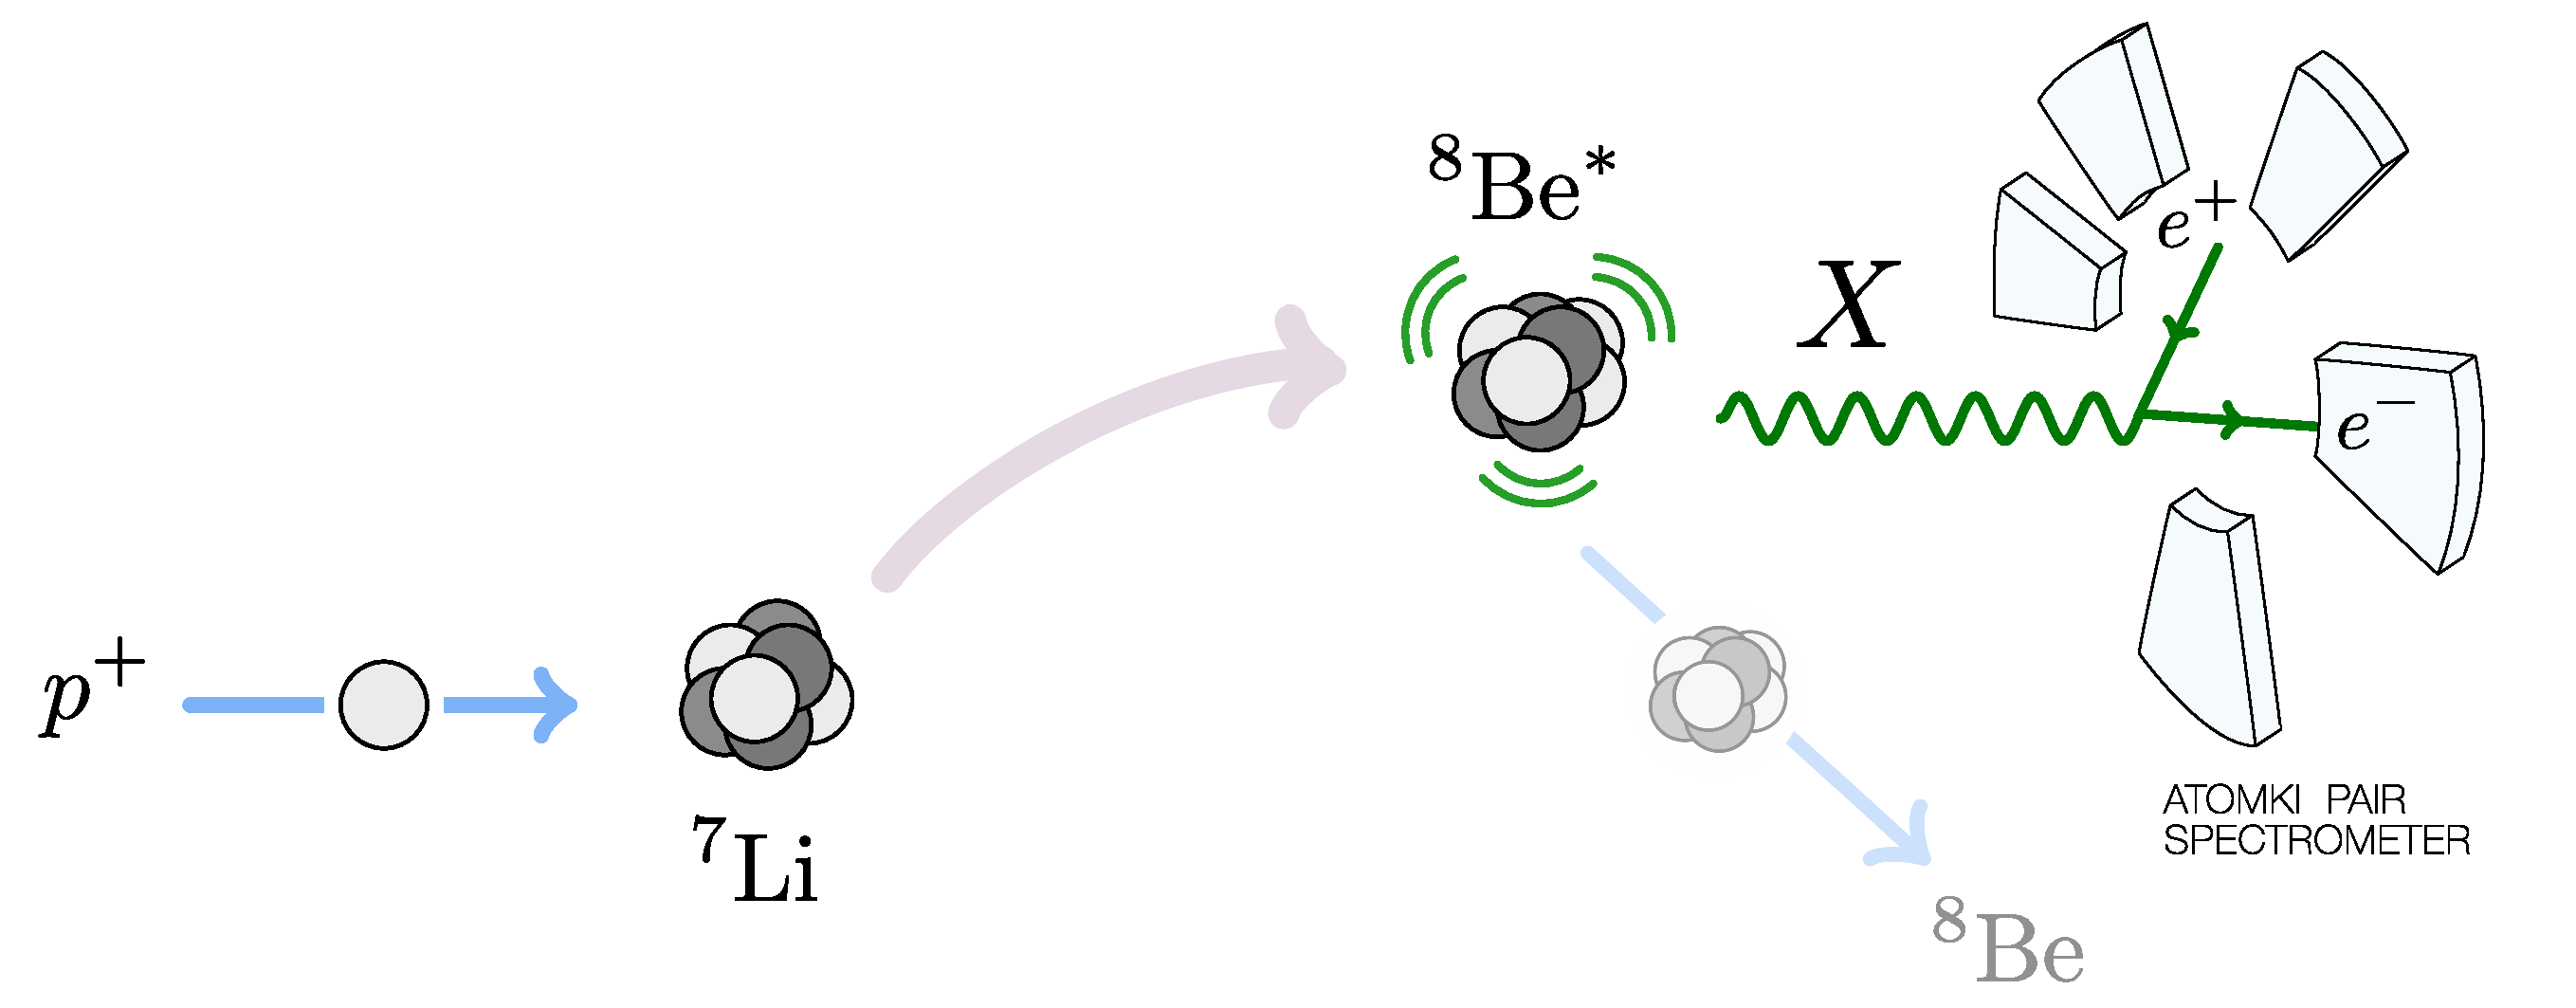
\includegraphics[width=.75\textwidth]{IPCArtistLong}
	\end{center}
	\caption{This is a figure.
	\label{fig:IPC}}
\end{figure}

And refer to Figure~\ref{fig:IPC}. It has nothing to do with Table~\ref{table:elements}.

\section*{Acknowledgements}


%This work is supported in part by 
%the \textsc{nsf} grant \textsc{phy}-1316792. 
%
\textsc{p.t.}\ thanks 
\emph{your name here}
for useful comments and discussions. 
%

%% Appendices
% \appendix


%% Bibliography
\bibliographystyle{utphys} 	% arXiv hyperlinks
%\bibliographystyle{utcaps} 	% arXiv hyperlinks
 \bibliography{FlipBib}
 


\end{document}